\section{Discussion}
For the previous genetic programming approach that did not incorporate modularization, results were compared to those in the existing literature \cite{owen1999tubular, luukka2009pca, dash2013comparative} and it was noted that - while additional research is necessary to explore the application of a GP approach using a larger data set - the classifiers produced by the genetic programming approach performed relatively well. For this assignment, modularization - in the form of automatically defined functions - has been added to the genetic programming approach to investigate its effect in terms of accuracy, computational effort and structural complexity. 

When compared to the results of the approach that did not incorporate modularization, the classifiers produced after adding modularization showed similar results in terms of accuracy. For instance, the best accuracy achieved on the training set before modularization was 87.14\% and, after modularization, this decreased slightly to 85.71\%. On the evaluation set, however, the best accuracy improved from 75\% to 80\% - indicating that introducing modularization may lead to better generalization.


% \begin{table}[H]
% \resizebox{\textwidth}{!}{\begin{tabular}{|c|c|c|c|}
% \hline
% \textbf{}               & \textbf{Average Accuracy} & \textbf{Best Accuracy} & \textbf{Standard Deviation} \\ \hline
% \textbf{Training Set}   & 83.71\%                   & 87.14\%                & 3.14\%                      \\ \hline
% \textbf{Evaluation Set} & 66.00\%                   & 75.00\%                & 6.63\%                      \\ \hline
% \textbf{Overall}        & 79.77\%                   & 82.22\%                & 2.43\%                      \\ \hline
% \end{tabular}}
% \caption{Classification Accuracy Before Modularization}
% \label{tab:classification_accuracy_before}
% \end{table}

In terms of computational effort, since no solutions were able to classify the data with a 100\% accuracy, it is unfortunately not possible to calculate how many programs have to be evaluated before a solution can be found. As an alternative for determining affects on computational effort, the runtimes for 10 test runs using the genetic programming approaches with and without modularization were recorded and are shown in figure \ref{fig:runtimes}. As can be seen, runtimes for the approach that incorporates modularization are consistently shorter than the previous approach. Considering the approaches used the same genetic algorithm parameters, this is a strong indicator that introducing modularization has decreased computational effort.

\begin{figure}[H]
\centering
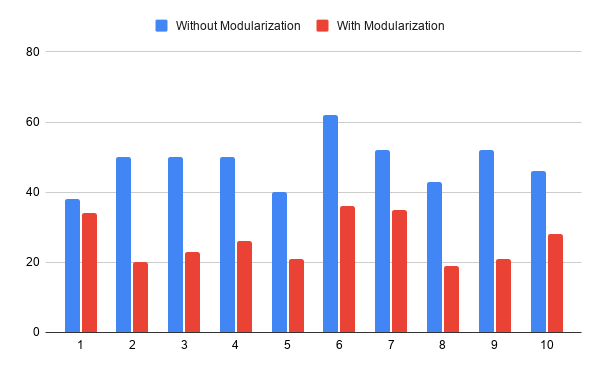
\includegraphics[width=\textwidth]{report/08_discussion/runtimes.png}
\caption{Runtimes for 10 Test Runs With and Without Modularization}
\label{fig:runtimes}
\end{figure}

Finally, in considering the structural complexity of individuals produced by either approach, we consider the number terminal and function nodes that individuals are composed of. For the approach that did not incorporate modularization, the fittest individuals for each of 10 test runs had an average of 48.11 terminal and function nodes. For the approach that did incorporate modularization, this average was 36.03. Hence, it would seem that the approach using modularization evolves towards less complex individuals. However, since only the best individual per test run was considered in this calculation, no conclusions are drawn regarding the complexity of individuals during the evolutionary process.

In conclusion, expanding the previous genetic programming approach to produce a classifier for postoperative patient diagnosis by adding modularization led to similar results in terms of accuracy and improvements in both computational effort and structural complexity.
